\documentclass{beamer}

\usepackage[utf8]{inputenc}
\usepackage{tikz}
\usepackage{bytefield}
\usepackage{pgf-umlsd}
\usepackage{mathpartir}

\usetikzlibrary{arrows,positioning,fit,shapes,automata}



\usetheme{Verona}

\title{Operational Semantics for VMs in Hafnium}
\institute{Aarhus University}
\date{\today}
\author[Liu, Stepanenko, Trieu, Birkedal]
{\underline{Z.~Liu}, S.~Stepanenko, A.~Trieu, L.~Birkedal}

\institute[Aarhus]
{
  Department of Computer Science\\
  Aarhus University
}

% notations
\newcommand*{\defined}{\triangleq}
\newcommand*{\maps}{\rightarrow}
\newcommand*{\derived}{::=}

% definitions
\newcommand*{\CONF}{\text{ExecConf}}
\newcommand*{\STATE}{\text{State}}
\newcommand*{\MEM}{\text{GlobalMem}}
\newcommand*{\SSS}{\text{ShareStates}}
\newcommand*{\PID}{\text{PID}}
\newcommand*{\PT}{\text{PageTable}}
\newcommand*{\AS}{\text{AccessState}}
\newcommand*{\OS}{\text{OwnershipState}}
\newcommand*{\REGS}{\text{Registers}}
\newcommand*{\ADDR}{\text{Address}}
\newcommand*{\WORD}{\text{Word}}
\newcommand*{\VMID}{\text{VMID}}
\newcommand*{\REGNAMES}{\text{RegisterName}}
\newcommand*{\MODE}{\text{ExecMode}}
\newcommand*{\DONE}{\text{DoneState}}
\newcommand*{\INSTR}{\text{Instruction}}
\newcommand*{\MB}{\text{MailBox}}

% parameters
\newcommand*{\PABITS}{\text{ADDR\_BITS}}
\newcommand*{\PPBITS}{\text{PAGE\_BITS}}
\newcommand*{\PPIDBITS}{\text{PID\_BITS}}
\newcommand*{\PAMAX}{\text{ADDR\_MAX}}
\newcommand*{\PPMAX}{\text{PAGE\_MAX}}
\newcommand*{\PPIDMAX}{\text{PID\_MAX}}
\newcommand*{\PWBITS}{\text{WORD\_BITS}}
\newcommand*{\PWMAX}{\text{WORD\_MAX}}
\newcommand*{\PVMMAX}{\text{VM\_MAX}}


% instructions
\newcommand*{\instrm}[1]{\mathtt{#1}}
\newcommand*{\instr}[1]{\texttt{#1}}

% expressions
\newcommand*{\EI}[1]{\mathtt{ExecInstr} \; {#1}}
\newcommand*{\RP}[1]{\mathtt{Repeat} \; {#1}}
\newcommand*{\DN}[1]{\mathtt{Done} \; {#1}}
\newcommand*{\NXT}[1]{\mathtt{Next} \; {#1}}

% functions
\newcommand*{\decode}{\text{decode}}
\newcommand*{\pid}{\text{pid}}
\newcommand*{\addr}{\text{addr}}

% SOME/NONE
\newcommand{\SOME}{\mathtt{Some}}
\newcommand{\NONE}{\mathtt{None}}

% TRUE/FALSE
\newcommand{\TRUE}{\mathtt{True}}
\newcommand{\FALSE}{\mathtt{False}}

\newcommand{\reg}[1]{\texttt{{#1}}}
\newcommand{\ta}[1]{\text{to\_addr}({#1})}
\newcommand{\tw}[1]{\text{to\_word}({#1})}
\newcommand{\tv}[1]{\text{to\_vmid}({#1})}
\newcommand{\DNNXT}[1]{\DN{\NXT{ {#1} }}}

\begin{document}

\frame{\titlepage}



% \begin{frame}
%   \frametitle{Settings of Hafnium}
%   \begin{figure}
% 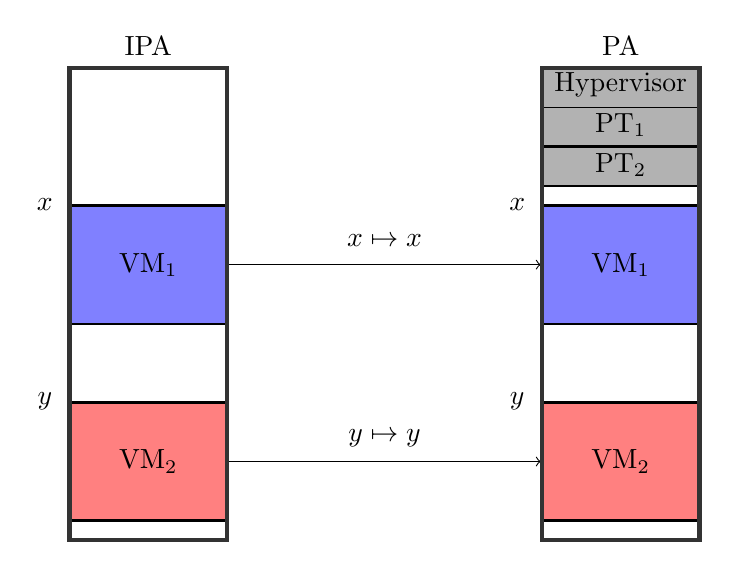
\begin{tikzpicture}[node distance=1cm, on grid]
 \tikzset{
pagetable/.style = {draw, minimum width=2cm,text height = 0.20cm},
memory/.style= {rectangle , draw = black, thick, minimum width = 2cm},
address space/.style = { rectangle, draw=black!80, ultra thick,minimum width=2cm,minimum height=6cm}}

\pgfdeclarelayer{foreground}
\pgfsetlayers{main,foreground}

    \begin{pgfonlayer}{foreground}
      \node [address space] (IPA)  at (-3,0) {};
      \node [address space] (PA) at (3,0) {};
      \node [above] at (PA.north) {PA};
      \node [above] at (IPA.north) {IPA};
    \end{pgfonlayer}
    \node [memory] (IP1)[fill = blue!50,minimum height = 1.5cm] at (-3,0.5) {VM$_{1}$};
    \node (X)[xshift = -3mm] at (IP1.north west) {$x$};
    \node [memory] (IP2)[fill = red!50,minimum height = 1.5cm] at (-3,-2) {VM$_{2}$};
    \node (Y)[xshift = -3mm] at (IP2.north west) {$y$};
    \node [memory] (PH)[fill = black!30,minimum height = 1.5cm] at (3,2.25) {};

    \node [pagetable] (PT1) at (3,2.25){PT$_{1}$};
    \node [pagetable] (PT2) at (3,1.75){PT$_{2}$};
    \node [above] at (PT1.north) {Hypervisor};

    \node [memory] (P1)[fill = blue!50,minimum height = 1.5cm] at (3,0.5) {VM$_{1}$}edge[<-] (IP1.east |- P1.west);
    \node (X')[xshift = -3mm] at (P1.north west) {$x$};
    \node [memory] (P2)[fill = red!50,minimum height = 1.5cm] at (3,-2) {VM$_{2}$}edge[<-] (IP2.east |- P2.west);
    \node (Y')[xshift = -3mm] at (P2.north west) {$y$};
    \node (E1)[minimum height = 0.5cm] at (0,0.8) {$x \mapsto x$};%edge[<-] (PT1.west);
    \node (E2)[minimum height = 0.5cm] at (0,-1.7) {$y \mapsto y$};%edge[<-] (PT2.west);

  \end{tikzpicture}

% \caption{Stage-2 Memory Translation}
% \end{figure}
% \end{frame}

\begin{frame}
  \frametitle{Settings of Hafnium}
  \begin{itemize}
    \item Simple translation regime, 1-to-1 mapping at stage 2
    \item Fixed number of VMs, loaded at boot time
    \item One primary+mutiple secondary, the scheduler resides in the primary
    \item Sequential world, only one physical CPU
    \item FF-A framework is deployed for intercommunication between VMs
    \item TLB, cache, I/O etc. are ommited
  \end{itemize}
\end{frame}

\begin{frame}
  \frametitle{FF-A framework}
  \begin{itemize}
    \item Implemented as synchronous exceptions by Hafnium (at EL2)
    \item \texttt{hvc} calling conventions
      \begin{itemize}
        \item parameter registers: \texttt{W0}-\texttt{W7}
          \item return registers: \texttt{W0}-\texttt{W3}
          \end{itemize}
    \item CPU cycle management
      \begin{itemize}
        \item FFA\_RUN - can only be invoked by the primary VM
        \item FFA\_YIELD - can be invoked by secondary VMs
        \item FFA\_MSG\_WAIT - block the caller until a message comes
      \end{itemize}

  \end{itemize}
\end{frame}


\begin{frame}
  \frametitle{FF-A framework}
  Message passing(indirect messaging, Hafnium is involved)
  \begin{itemize}
    \item RX page/TX page - read-only/write-only, states are monitored by Hafnium
    \item FFA\_MSG\_SEND - copy, notify the scheduler and the receiver
    \item FFA\_MSG\_POLL - return error if no message is ready in RX
  \end{itemize}
  \begin{figure}
    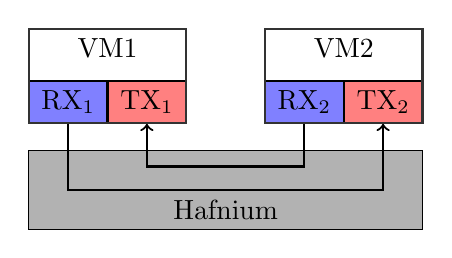
\begin{tikzpicture}[node distance=1cm, on grid]
\usetikzlibrary{arrows,positioning,fit,shapes}
 \tikzset{
Hypervisor/.style = {draw, minimum width=5cm},
page/.style= {rectangle , draw = black, thick, minimum width = 1cm,minimum height =0.5 cm},
VM/.style = { rectangle, draw=black!80, thick,minimum width=2cm,minimum height=1.2cm}}

\pgfdeclarelayer{foreground}
\pgfsetlayers{main,foreground}

    \begin{pgfonlayer}{foreground}
      \node [VM] (VM1)  at (-1.5,0.75) {};
      \node [VM] (VM2) at (1.5,0.75) {};
      \node [above,yshift=-0.5cm] at (VM1.north) {VM1};
      \node [above,yshift=-0.5cm] at (VM2.north) {VM2};
    \end{pgfonlayer}
     \node [page] (RX1)[fill = blue!50,] at (-2,0.42) {RX$_1$};
     \node [page] (TX1)[fill = red!50] at (-1,0.42) {TX$_{1}$};
      \node [page] (RX2)[fill = blue!50] at (1,0.42) {RX$_2$};
     \node [page] (TX2)[fill = red!50] at (2,0.42) {TX$_{2}$};

     \node [Hypervisor] (Hyp)[fill = black!30,minimum height = 1cm] at (0,-0.7) {};
     \node [below,yshift=0.5cm] at (Hyp.south) {Hafnium};


      \coordinate (P1) at (-2,-0.7);
      \coordinate (P2) at (-1,-0.4);
      \coordinate (P3) at (2,-0.7);
      \coordinate (P4) at (1,-0.4);

      \draw [thick,->]  (RX1.south) |- (P1) -- (P3)-|  (TX2.south);
      \draw [thick, ->]  (RX2.south) |- (P4) -- (P2)-|  (TX1.south);

  \end{tikzpicture}

        \caption{Indirect messaging with RX/TX}
      \end{figure}
\end{frame}

\begin{frame}
  \frametitle{FF-A framework}
  Memory management
  \begin{itemize}
    \item All about ownership and access...
    \item Donation - sender loses ownership and access
    \item Sharing - sender keeps ownership and access
    \item Lending - sender loses access but keeps ownership
    \item FFA\_MEM\_RELINQUISH - receiver gives up access
    \item FFA\_MEM\_RECLAIM - sender regains exclusive access
    \item FFA\_MEM\_RETRIEVE\_REQUEST - receiver gets access/ownership
  \end{itemize}
  \begin{figure}
    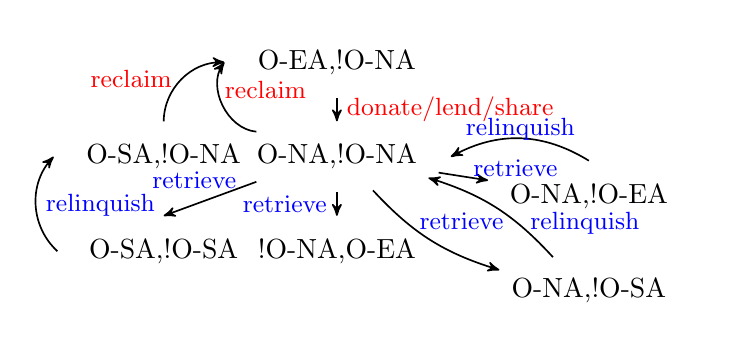
\begin{tikzpicture}[->,>=stealth',auto,node distance=1.2cm, semithick]
  \tikzstyle{every state}=[ellipse,draw=none,text=black,scale =1,inner sep=0pt]

  \node[state] (A)                    {O-EA,!O-NA};
  \node[state] (B) [below of= A]      {O-NA,!O-NA};
  \node[state] (C1) [below of= B]      {!O-NA,O-EA};
  \node[state] (C2) [left of= C1,xshift=-1cm]      {O-SA,!O-SA};
  \node[state] (C3) [right of= B,xshift=2cm,yshift=-0.5cm]      {O-NA,!O-EA};
  \node[state] (C4) [below of= C3]      {O-NA,!O-SA};
\node[state] (B2) [left of= B,xshift=-1cm]      {O-SA,!O-NA};

  \path (A.south) edge node[color=red] {\small donate/lend/share} (B.north)
  (B.south) edge node[color=blue,left] {\small retrieve} (C1.north)
  (B.south west) edge node[color=blue,above,xshift=-0.2cm] {\small retrieve} (C2.north)
  (B) edge[bend right = 0] node[color=blue,right,yshift=0.1cm] {\small retrieve} (C3)
  (C3.north) edge[bend right] node[color=blue,above,yshift=-0.15cm] {\small relinquish} (B.east)
  (B) edge[bend right=15] node[color=blue,above,xshift=0.4cm,yshift=0cm] {\small retrieve} (C4)
  (C2.west) edge[bend left=45] node[color=blue,right,xshift=0cm] {\small relinquish} (B2.west)
  (B2.north) edge[bend left=45] node[color=red,left,xshift=0cm] {\small reclaim} (A.west)
  (B.north west) edge[bend left=60] node[color=red,right,xshift=-0.1cm,yshift=0.2cm] {\small reclaim} (A.west)
  (C4) edge[bend right=15] node[color=blue,right,xshift=0.3cm,yshift=-0.2cm] {\small relinquish} (B)
  ;
\end{tikzpicture}

        \caption{ownership and access}
      \end{figure}
    \end{frame}

\begin{frame}
  \frametitle{FF-A framework}
\begin{columns}[T] % align columns
\begin{column}{.58\textwidth}
  Memory management
  \begin{itemize}
    \item Three steps for one completed transaction
    \item Transaction descriptor, transfered via RX\&TX
  \end{itemize}
  \begin{figure}
    \begin{sequencediagram}
      \tikzstyle{inststyle}=[]
     \newinst{Hyp}{\small{Hypervisor}}
     \newinst[1]{VM0}{\small{VM 0}}
     \newinst[1]{VM1}{\small{VM 1}}

\addtocounter{seqlevel}{-1}
     \begin{messcall}{VM0}{\tiny{donate page $p$ to 1}}{Hyp}

     \end{messcall}
     \addtocounter{seqlevel}{-1}
     \begin{messcall}{VM0}{\tiny{donated page $p$ to you}}{VM1}
     \end{messcall}
     \addtocounter{seqlevel}{-1}
     \begin{messcall}{VM1}{\tiny{retrieve the page $p$ that 0 donated to me}}{Hyp}
     \end{messcall}
     \addtocounter{seqlevel}{-1}

 \end{sequencediagram}
        \caption{Three steps for donation}
      \end{figure}
\end{column}%
\hfill%
\begin{column}{.38\textwidth}
 \begin{figure}
    \vspace{0pt}
\begin{minipage}{\textwidth}
      \begin{bytefield}[rightcurlyspace=0pt,bitheight=2.5ex]{8}
        \wordbox{1}{Sndr VMID}\\
        \wordbox{1}{Flag}\\
        \wordbox{1}{Handle}\\
     %   \wordbox{1}{Tag}\\
        \wordbox{1}{Counter $c$}\\
        \begin{rightwordgroup}{$c$}
        \wordbox{1}{Rcvr VMID 1}\\
        \wordbox{1}{Offset 1}\\
        \skippedwords
        \end{rightwordgroup}\\
        \begin{rightwordgroup}{Offset 1}
          \wordbox{1}{Counter $n_{1}$}
        \end{rightwordgroup}\\
        \begin{rightwordgroup}{$n_{1}$}
            \wordbox{1}{PID $1_1$}\\
            \skippedwords
            \end{rightwordgroup}\\
\end{bytefield}
\end{minipage}%
        \caption{Layout of the (simplified) descriptor}
      \end{figure}
\end{column}%
\end{columns}

\end{frame}

\begin{frame}
  \frametitle{Execution Configuration}
\begin{figure}
  \begin{align*}
    \Phi &\in \CONF &\defined &\text{States} \times \MEM \times \SSS \\
    \delta s &\in \text{States} &\defined &\text{list(States)} \\
    \delta &\in \STATE &\defined &\PT \times \REGS \times \MB \\
    pt & \in \PT & \defined & \PID \maps (\OS \times \AS) \\
    mb & \in \MB &\defined &\text{TXPage} \times  \text{RXPage}\\
    tx & \in \text{TXPage} &\defined &\PID\\
    rx & \in \text{RXPage} &\defined &\PID \times \text{Bool} \times \WORD \times \VMID \\
    pid & \in \PID &\defined  &[ 0, \PPIDMAX ] \\
     v,n & \in \VMID &\defined  &[ 0, \PVMMAX ] \\
      & \;\;\;\; \OS & \derived & O | !O  ~~~~~~~  \AS  \derived  NA | EA | SA
  \end{align*}
  \caption{Execution Configuration: VM States.}
\end{figure}

\end{frame}

\begin{frame}
  \frametitle{Execution Configuration}
\begin{figure}
  \begin{align*}
      rs & \in \REGS &\defined  &\REGNAMES \maps \WORD \\
    rn & \in \REGNAMES &\defined &\text{SysRegs} \cup \text{GenRegs}\\
    mm & \in \MEM &\defined  &\ADDR \maps \WORD \\
    a & \in \ADDR &\defined  &[ 0, \PAMAX ] \\
    w & \in \WORD &\defined  &[ 0, \PWMAX ] \\
    sss & \in \SSS &\defined  &\WORD \maps \text{ShareState} \\
    ss & \in \text{ShareState} &\defined &\VMID \times \WORD \times \WORD \times\\
                                        &&&   [\VMID] \times (\VMID \maps [\PID]) \times \text{FunctionID}\\
      & \;\;\;\; \text{SysRegs} &\derived & \mathtt{NV} | \mathtt{CNT\_VAL} | \mathtt{CNT\_CTL} | \dots \\
         & \;\;\;\; \text{GenRegs} &\derived & \mathtt{pc} | \mathtt {R0} | \mathtt{R1} | \dots
  \end{align*}
  \caption{Execution Configuration: Global Memory and Share States.}
\end{figure}

\end{frame}


\begin{frame}
  \frametitle{Syntax and Instructions}
\begin{figure}
  \begin{align*}
    \mu &\in \MODE &\derived & \mathtt{ExecInstr} \; v | \mathtt{Repeat} \; \mu | \mathtt{Done} \; \theta \\
    \theta &\in \DONE &\derived & \NXT{v} | \mathtt{Halt} | \mathtt{Fail}\\
    \\
    instr & \in  \INSTR &\derived & \instrm{br} \; r |\instrm{bne} \; r \; r |
                                    \instrm{mov} \; r \; w | \instrm{ldr} \; r\; r|
                                    \instrm{str} \; r \; r | \instrm{add} \; r \; r \; r \\
        & & & | \instrm{sub} \; r \; r \; r | \instrm{cmp} \; r \; r | \instrm{fail} | \instrm{halt} | \instrm{hvc} |\instrm{mrs} \; r\;r | \instrm{msr} \; r \; r\\
    fid & \in \text{FunctionID} &\derived & \tt{RUN} ~|~\tt{YIELD} ~|~\tt{MSG\_WAIT} ~|~\tt{MSG\_SEND}
                                            ~|~\tt{MSG\_POLL}~ \\
        &&&|~\tt{MEM\_DONATE}~|~\tt{MEM\_RETRIEVE\_REQ} ~|~ \tt{SUCC} ~|~\tt{ERROR}\\
        &&&|~\tt{MEM\_RETRIEVE\_RESP}~|~\tt{MEM\_SHARE} ~|~ \tt{MEM\_LEND}\\
        &&&|~\tt{MEM\_RECLAIM}~|~\tt{MEM\_RELINQUISH}\\
    err & \in \text{ErrorCode} &\derived & \tt{INV\_PARA} ~|~\tt{DENIED} ~|~\tt{BUSY}~|~\tt{RETRY}
  \end{align*}
  \caption{Syntax and machine instructions}
\end{figure}

\end{frame}

\begin{frame}
  \frametitle{Rules(Selected)}
\begin{figure}[!htb]
  \begin{mathpar}
    \inferrule[RepeatExec] {(\EI{v},\, \phi) \rightarrow (\DN{\theta} ,\,
      \phi')} {(\RP{\EI{v}} ,\, \phi) \rightarrow (\RP{\DN{\theta}} ,\, \phi')}
    \and \inferrule[RepeatHalt/Fail] {\theta = \mathtt{Halt} \lor \theta =
      \mathtt{Fail}} {(\RP{\DN{\theta}} ,\, \phi) \rightarrow (\DN{\theta} ,\,
      \phi)}
    \and \inferrule[RepeatNext]{} {(\RP{\DN{\NXT{v}}} ,\, \phi)
      \rightarrow (\RP{\EI{v}} ,\, \phi)}
  \end{mathpar}
  \caption{Reduction steps}
\end{figure}
\end{frame}

\begin{frame}
  \frametitle{Rules(Selected)}
  \begin{figure}
  \begin{mathpar}
    \inferrule[Fail-UnaccessibleInstr]
    {!\text{AccessibleAddr}(\delta_v,a_i)}
    {(\EI{v} ,\, \Phi) \rightarrow (\DN{\tt{Fail}} ,\, \Phi)}

    \inferrule[Exec-halt]
    {\text{AccessibleAddr}(\delta_v,a_i) \\\text{DecodeInstr}(\Phi.mm[a_i],\mathtt{halt})}
    {(\EI{v} ,\, \Phi) \rightarrow (\DN{\tt{Halt}} ,\, \Phi)}

    \inferrule[Exec-mov-Succ]
    {\text{AccessibleAddr}(\delta_v,a_i) \\\text{DecodeInstr}(mm[a_i],\mathtt{mov}~rn~w) \\ rn\in \text{GenRegs}}
    {(\EI{v} ,\,(\delta s,mm,sss)) \rightarrow \\ (\DNNXT{v} ,\, (\delta s \text{ with }\{ [v].rs[rn]=w ; [v].rs[\reg{pc}]=rs_v[\reg{pc}]+1\},mm,sss))}
  \end{mathpar}
  \caption{Rules for basic instructions}
  \end{figure}
\end{frame}

\begin{frame}
  \frametitle{Rules(Selected)}
  \begin{figure}
\begin{mathpar}

    \inferrule[Exec-hvc-Succ-MemMng-Succ-NotZeroed]
    {\text{AccessibleAddr}(\delta_v,a_i) \\
    \text{DecodeInstr}(mm[a_i],\mathtt{hvc}) \\
    \text{IsFFA}(\delta_v,f)\\
    f \in \{\tt{MEM\_SHARE}, \tt{MEM\_LEND}\} \\
    w_l = rs_v[\reg{R1}]\\
    pid_t=\delta_v.mb.tx\\
    \text{ValidTransactionDescriptor}(pid_t,w_l,v,0,0,w_t,w_c,pgs,mm,\delta s)\\
    w_h \notin \text{dom}(sss) \\
    w_h[63]=1\\
    }
    {(\EI{v} ,\,(\delta s,mm,sss)) \rightarrow (\DNNXT{v} ,\,\\ (\delta s \text{ with }\left\{{\begin{array}{l}
    [v].rs[\reg{pc}]=rs_v[\reg{pc}]+1;\\
    \null[v].rs[\reg{R0}]=\efid{SUCC};\\
    \null[v].rs[\reg{R2}]=w_h;\\
    \null \forall pid. \exists v_r. pid \in pgs[v_r] \rightarrow [v].pt[pid]=(O,NA);\\
    \null \forall pid. \exists v_r. pid \in pgs[v_r] \rightarrow [v_r].pt[pid]=(!O,NA)
    \end{array}}\right\},\\mm, sss~\text{with}~\{[w_h]=(v,0,w_t,[],pgs,f)\}))}
\end{mathpar}
  \caption{Rule for Memory Management}
  \end{figure}
\end{frame}

\begin{frame}
  \frametitle{Next Steps...}
  \begin{itemize}
    \item Include interrupts - crucial for scheduling
    \item Develope a program logic - to reason about client programs
    \item Investigate in security - confidentiality, isolation etc.
  \end{itemize}
\end{frame}




\end{document}
